%======================================================================
% CAPITULO 4: SEGURIDAD Y POLITICAS
%======================================================================

\chapter{Seguridad y Politicas de Proteccion}
\label{ch:seguridad}

La seguridad es el pilar fundamental de \sdc{}. Este capitulo detalla la configuracion de politicas de seguridad, gestion de contrasenas, niveles de auditoria y configuracion de rutas proxy seguras.

\section{Configuracion de Seguridad}
\label{sec:config-seguridad}

El panel de seguridad centraliza todas las configuraciones relacionadas con la proteccion del sistema y los datos.

\begin{figure}[H]
\centering
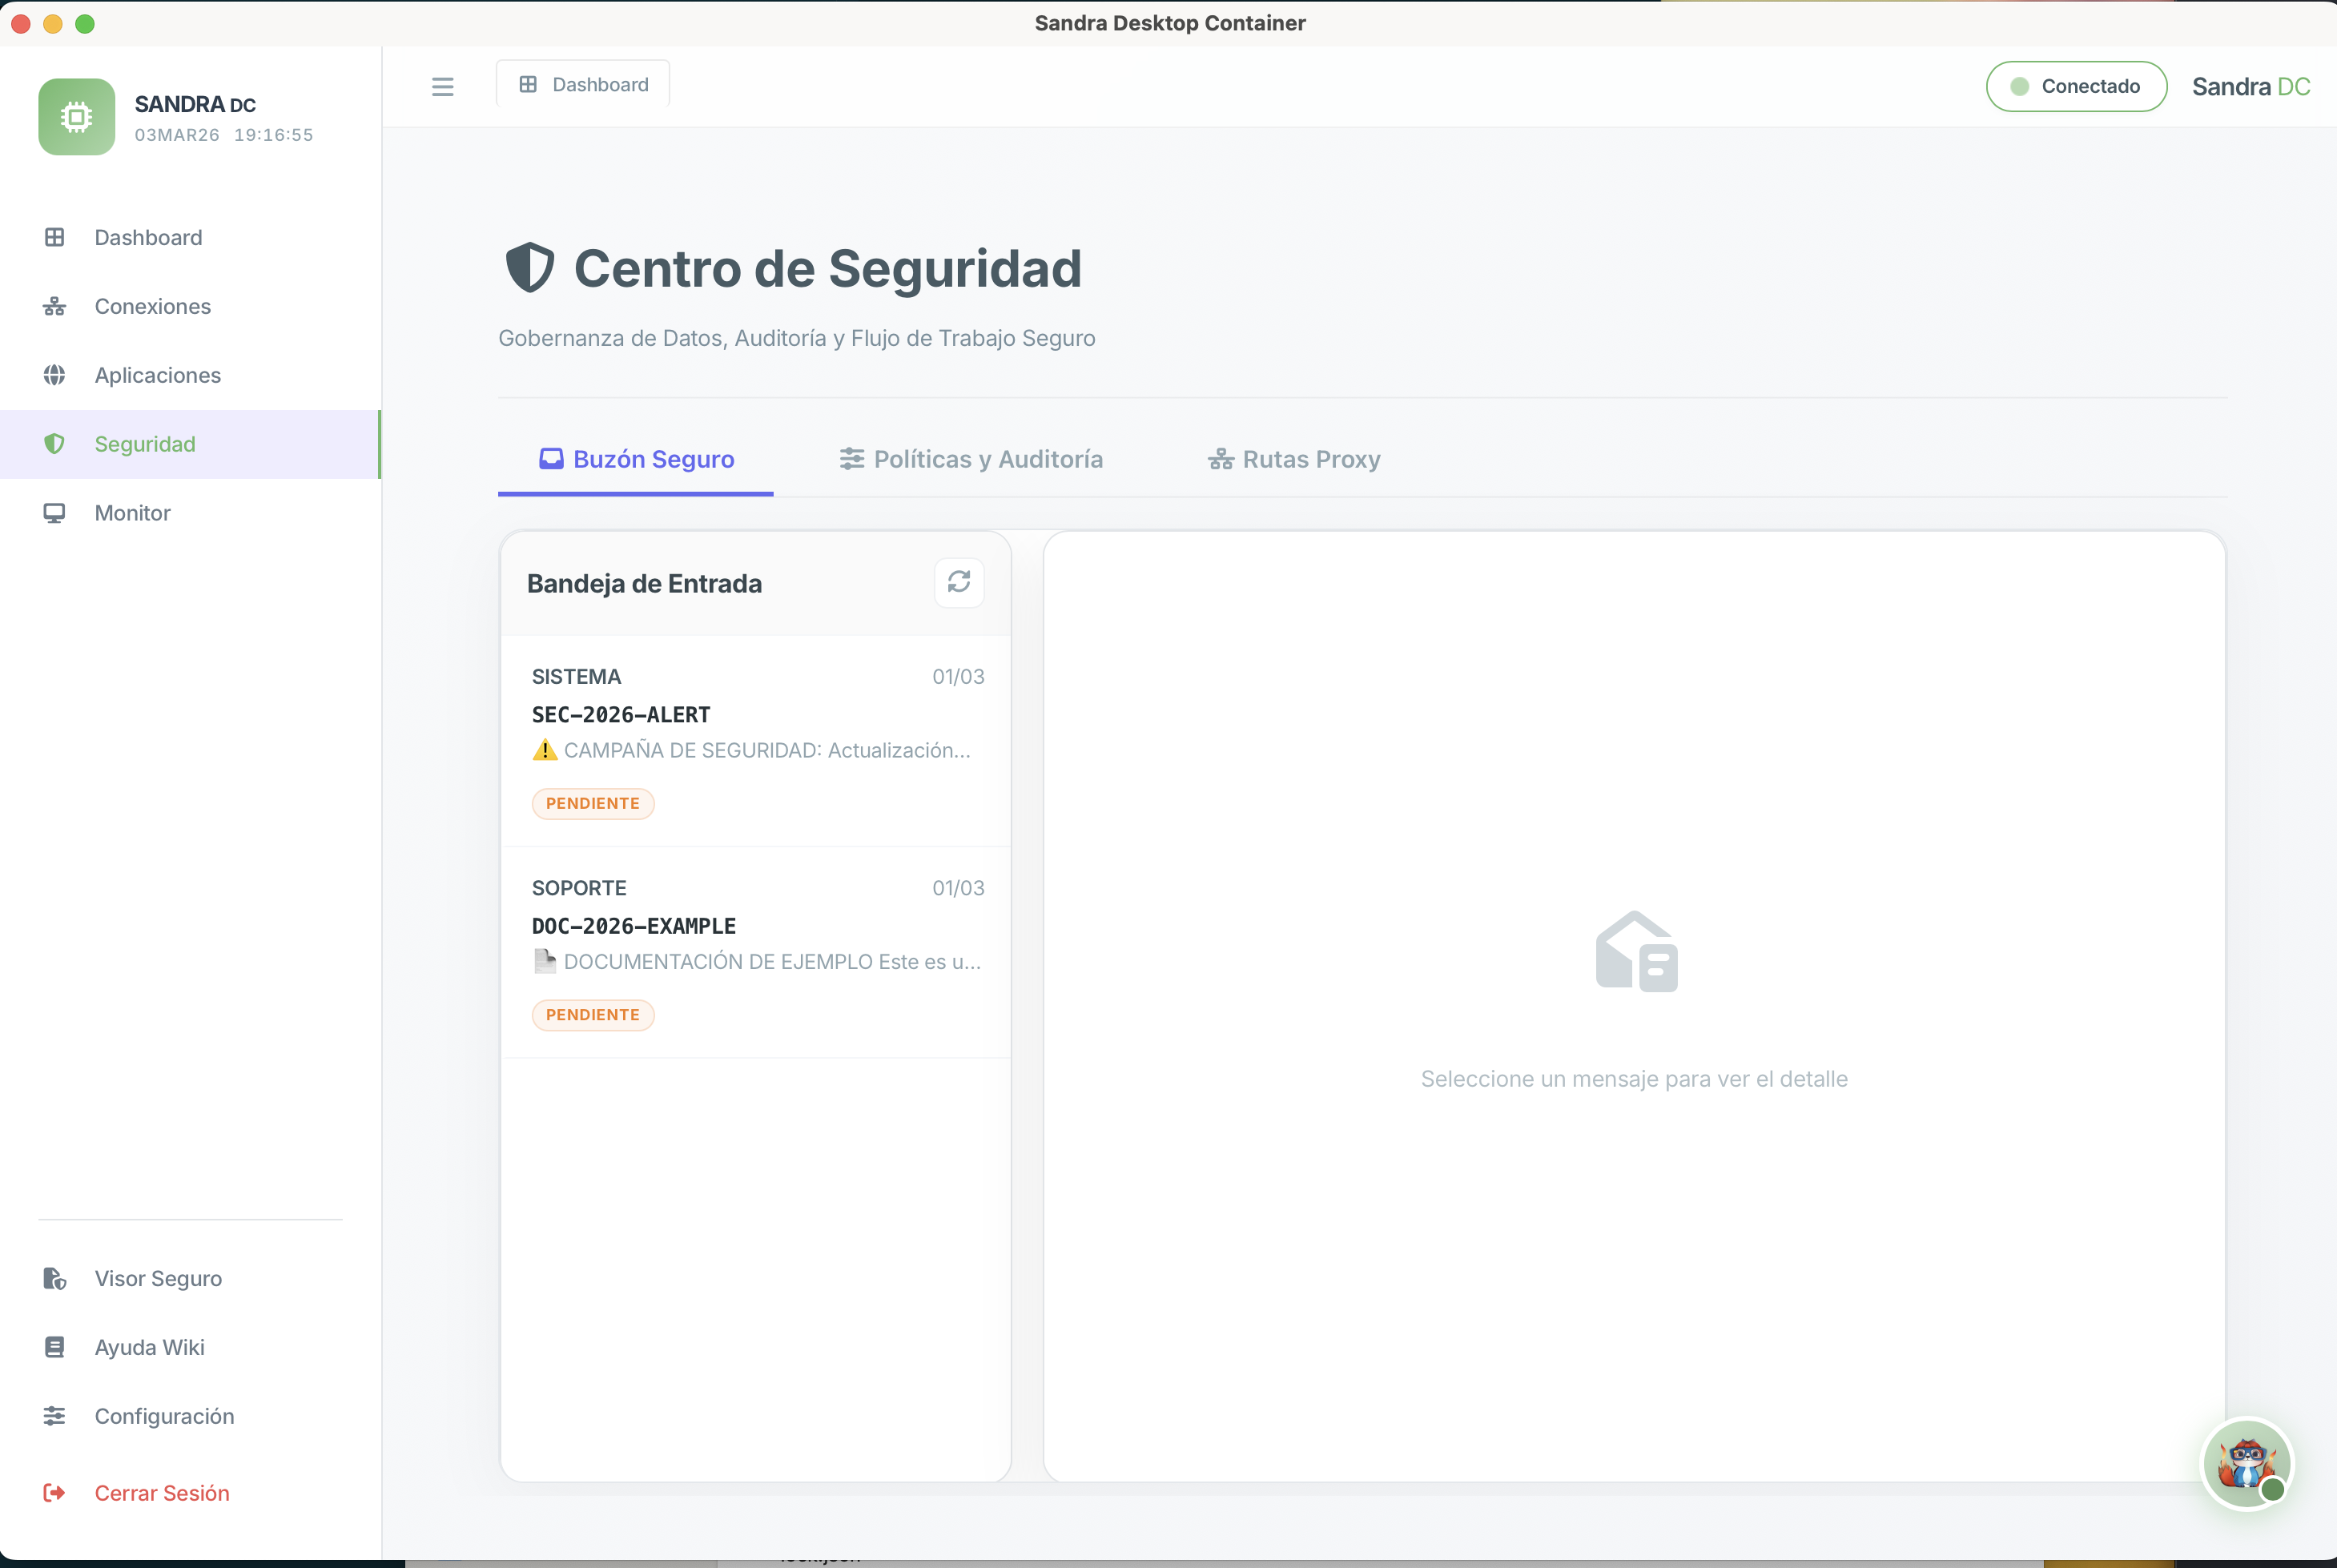
\includegraphics[width=0.95\textwidth]{anexos/7 seguridad.png}
\caption{Panel principal de configuracion de seguridad}
\label{fig:seguridad}
\end{figure}

\subsection{Niveles de Seguridad Predefinidos}

SDC ofrece tres perfiles de seguridad:

\begin{table}[H]
\centering
\begin{tabular}{p{3cm}p{5cm}p{5cm}}
\toprule
\textbf{Nivel} & \textbf{Caracteristicas} & \textbf{Recomendado Para} \\
\midrule
Basico & Auditoria minima, politicas estandar, logs locales & Entornos de desarrollo \\
\midrule
Estandar & Auditoria completa, contrasenas robustas, encriptacion AES-256 & Operaciones empresariales \\
\midrule
Critico & Auditoria en tiempo real, contrasenas de alta entropia, MFA, logs inmutables & Datos clasificados \\
\bottomrule
\end{tabular}
\caption{Niveles de seguridad predefinidos}
\label{tab:niveles-seguridad}
\end{table}

\section{Politicas de Contrasenas}
\label{sec:politicas-password}

Las politicas de contrasenas permiten definir expresiones regulares (regex) que validan la complejidad de las credenciales.

\begin{figure}[H]
\centering
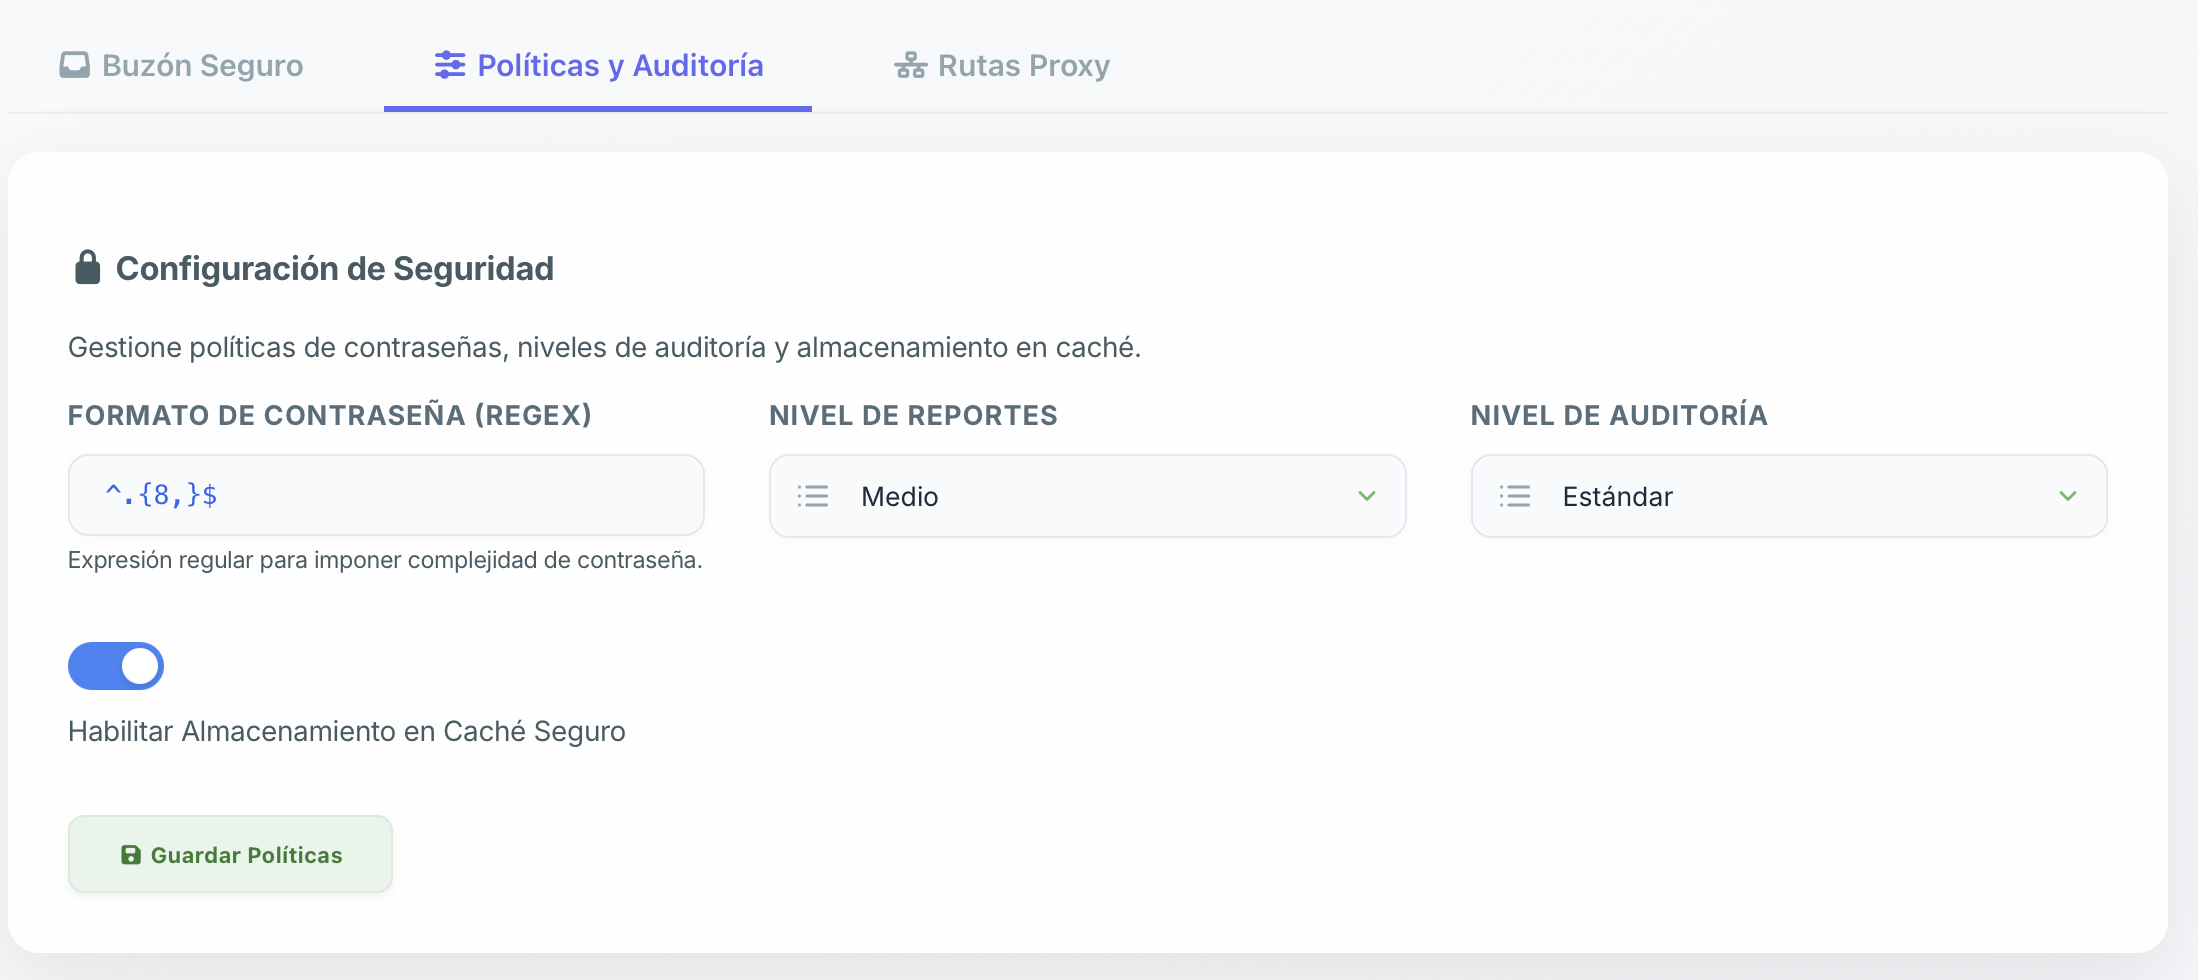
\includegraphics[width=0.95\textwidth]{anexos/8 politica.png}
\caption{Configuracion de politicas de contrasenas}
\label{fig:politicas}
\end{figure}

\subsection{Configuracion de Regex}

\begin{lstlisting}[language=bash, caption={Ejemplos de Regex para Contrasenas}]
# Basica: Minimo 8 caracteres
^(?=.{8,}).*$

# Estandar: 8+ chars, mayuscula, minuscula, numero
^(?=.*[a-z])(?=.*[A-Z])(?=.*\d).{8,}$

# Critica: 12+ chars, mayuscula, minuscula, numero, especial
^(?=.*[a-z])(?=.*[A-Z])(?=.*\d)(?=.*[@$!%*?&]).{12,}$

# Militar: 16+ chars, todos los tipos, sin repetidos
^(?=.*[a-z])(?=.*[A-Z])(?=.*\d)(?=.*[@$!%*?&])(?!.*(.)\1).{16,}$
\end{lstlisting}

\subsection{Algoritmo de Hashing}

Las credenciales nunca se almacenan en texto plano. SDC utiliza Argon2id para el hashing de contrasenas:

\begin{quote}
\textbf{Argon2id}\\
Argon2 es el ganador de la Password Hashing Competition (2015). La variante Argon2id ofrece resistencia a ataques de GPU y ASIC, y proteccion contra ataques de canal lateral.
\end{quote}

\begin{itemize}
    \item Memoria: 64 MB por operacion de hash
    \item Iteraciones: 3 passes
    \item Paralelismo: 4 threads
    \item Sal: 128 bits aleatorios unicos por contrasena
\end{itemize}

\section{Rutas Proxy}
\label{sec:rutas-proxy}

Las rutas proxy definen puntos de acceso seguro para los servicios expuestos por los contenedores.

\begin{figure}[H]
\centering
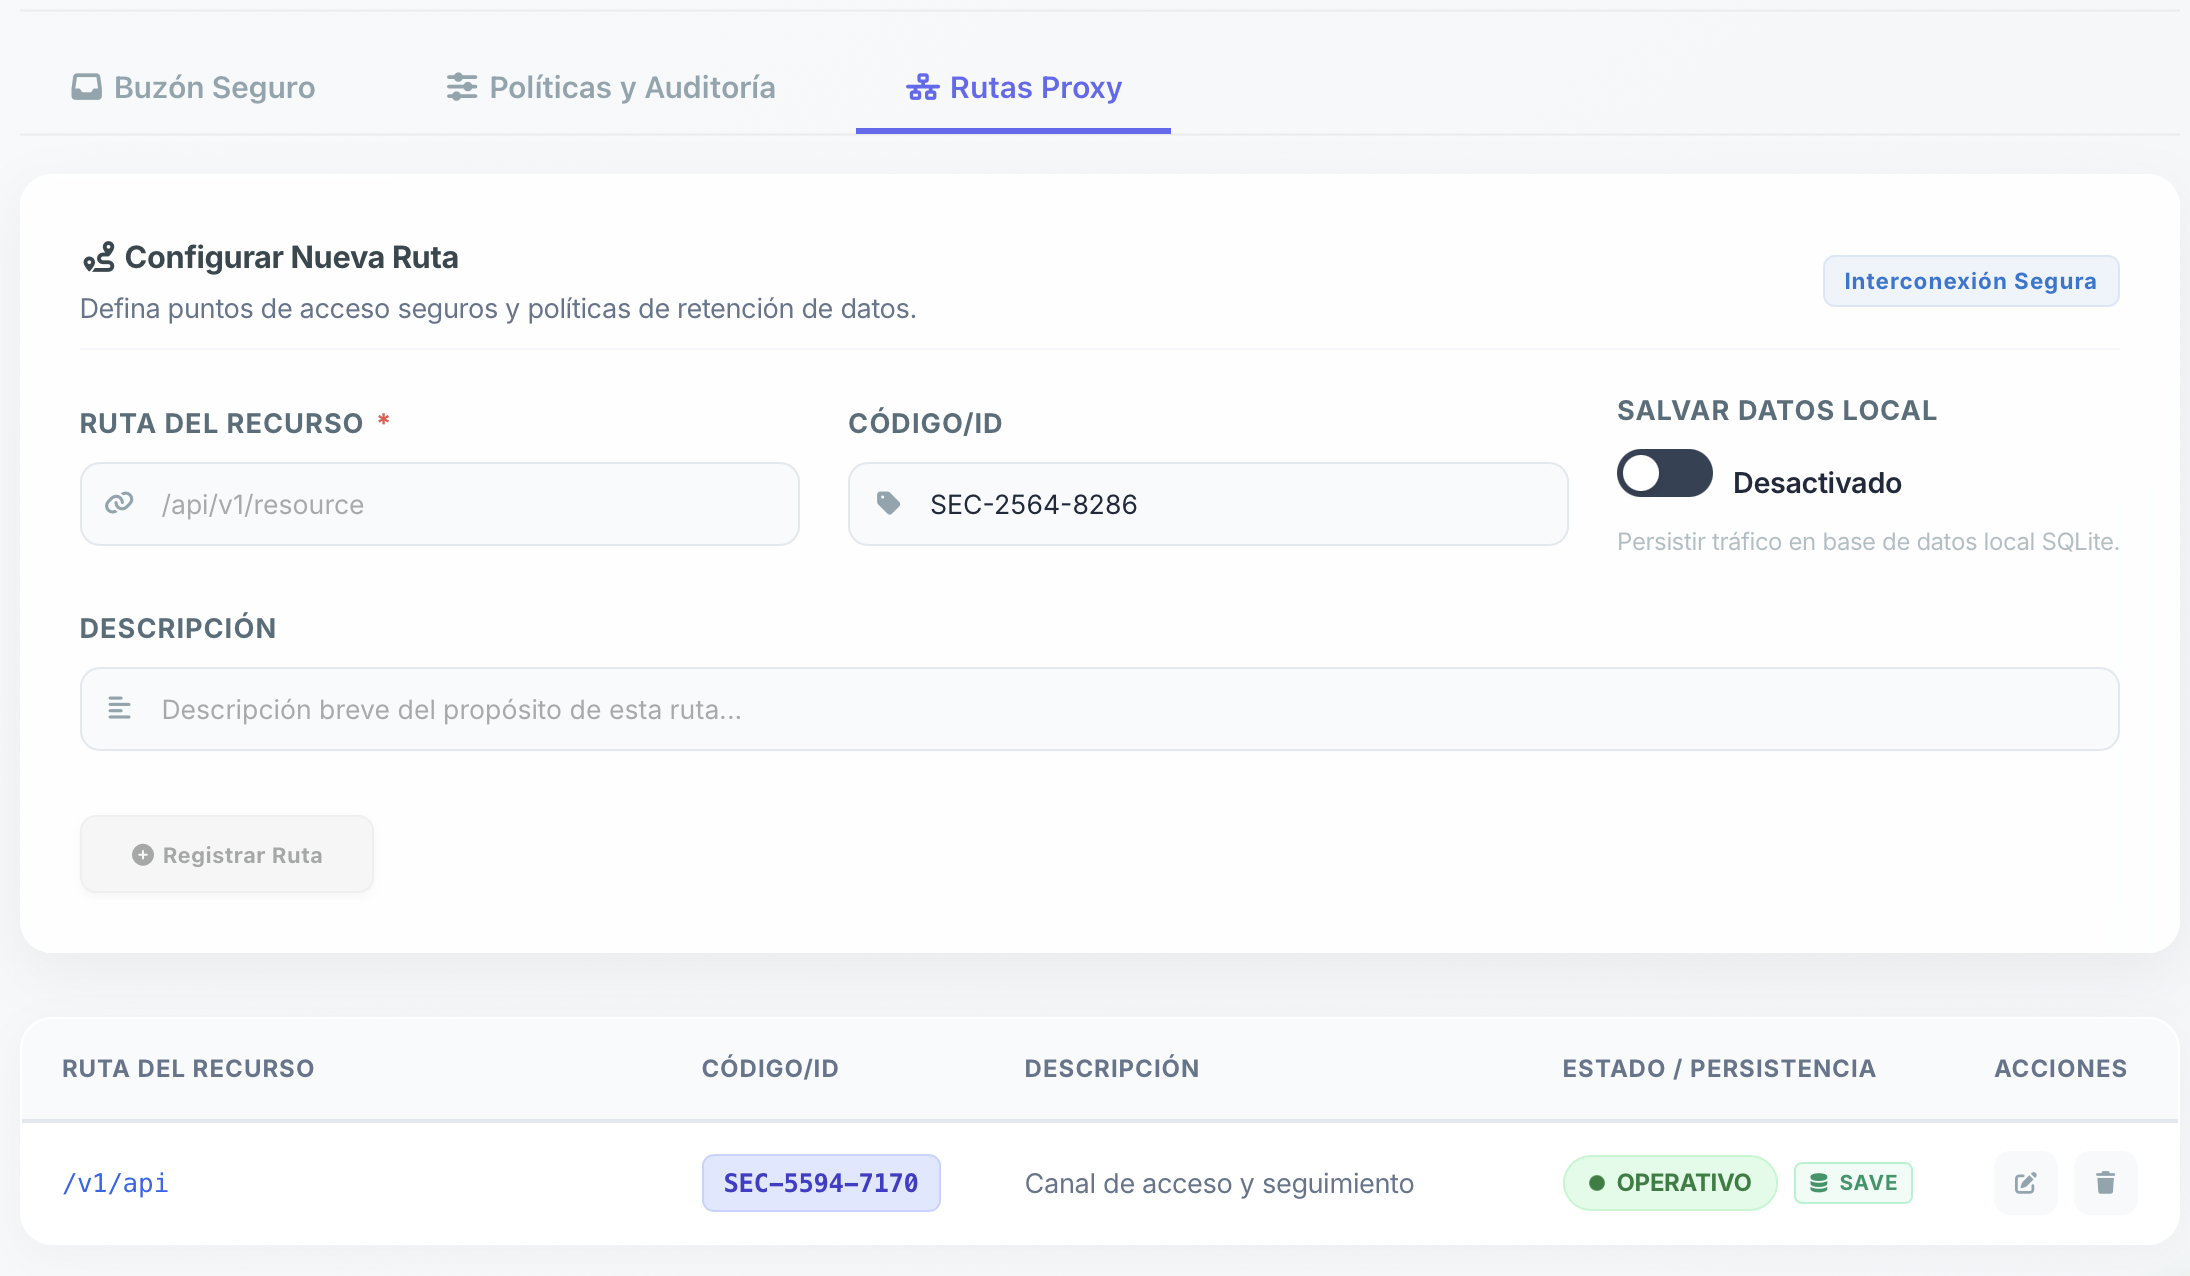
\includegraphics[width=0.95\textwidth]{anexos/9 proxy.png}
\caption{Gestor de rutas proxy}
\label{fig:proxy}
\end{figure}

\subsection{Creacion de Rutas}

Para cada ruta creada (ejemplo: /v1/api), SDC:

\begin{enumerate}[leftmargin=*]
    \item Genera un Codigo ID de Seguridad unico
    \item Configura el enrutamiento interno
    \item Establece politicas de acceso
    \item Opcionalmente, activa persistencia encriptada
\end{enumerate}

\subsection{Codigo ID de Seguridad}

El Codigo ID es un identificador criptografico que:

\begin{itemize}[leftmargin=*]
    \item Vincula la ruta a un Client ID especifico
    \item Incluye timestamp de creacion para expiracion opcional
    \item Se firma con la clave privada del nodo
    \item Se puede revocar individualmente
\end{itemize}

\subsection{Persistencia de Trafico}

\begin{quote}
\textbf{Encriptacion de Datos Persistentes}\\
Cuando la persistencia esta activada, todo el trafico se almacena localmente encriptado con AES-256-GCM. La clave de cifrado se deriva del Client ID mediante HKDF.
\end{quote}

\section{Auditoria y Logs}
\label{sec:auditoria}

SDC mantiene un registro inmutable de todas las operaciones.

\subsection{Niveles de Auditoria}

\begin{table}[H]
\centering
\begin{tabular}{p{3cm}p{4cm}p{6cm}}
\toprule
\textbf{Nivel} & \textbf{Eventos Registrados} & \textbf{Retencion} \\
\midrule
Basico & Inicio/cierre de sesion, errores criticos & 30 dias \\
\midrule
Estandar & Cambios de configuracion, accesos a documentos & 90 dias \\
\midrule
Critico & Todo trafico de red, queries de BD, IPC & 1 ano \\
\bottomrule
\end{tabular}
\caption{Niveles de auditoria y retencion de logs}
\label{tab:niveles-auditoria}
\end{table}

\subsection{Estructura de Logs}

\begin{lstlisting}[language=bash, caption={Formato de Log de Auditoria}]
{
  "timestamp": "2026-03-03T14:32:18.423Z",
  "level": "INFO",
  "client_id": "a1b2c3d4-e5f6...",
  "node_name": "sandra.produccion",
  "event": "DOCUMENT_ACCESS",
  "resource": "/docs/confidencial.pdf",
  "action": "VIEW",
  "result": "SUCCESS",
  "metadata": {
    "ip_source": "192.168.1.100",
    "session_id": "sess-xyz789"
  },
  "hash": "sha256:abc123...",
  "signature": "sig:def456..."
}
\end{lstlisting}

\section{Arquitectura de Defensa en Profundidad}

La seguridad de SDC se organiza en multiples capas:

\begin{enumerate}
    \item \textbf{Perimetro}: Firewall + WSS/TLS 1.3
    \item \textbf{Autenticacion}: Argon2id + MFA
    \item \textbf{Autorizacion}: RBAC + Rutas Proxy
    \item \textbf{Datos}: AES-256-GCM en reposo y transito
    \item \textbf{Auditoria}: Logs inmutables + Firma digital
\end{enumerate}
